\documentclass{beamer}
\usetheme[bgphoto]{polimi}
% Usage instructions can be found at: https://github.com/elauksap/beamerthemepolimi

\usepackage{tikz}
\usepackage{media9}
\usepackage[top=1in,bottom=1in,right=1in,left=1in]{geometry}
%\usepackage[utf8]{inputenc}
\usepackage{hyperref}
\usepackage{lipsum}
\usepackage{subcaption}
\usepackage{cancel}
\usepackage{graphicx}
\usepackage{caption}
\usepackage[backend=biber]{biblatex}
\usepackage{amsmath}
\usepackage{mathtools}
\addbibresource{main.bib}

\usepackage{tabularx}
\usepackage{longtable} % tables that can span several pages
\usepackage{colortbl}
\usepackage{booktabs}
\usepackage{wrapfig}
\usepackage{graphicx}


\pdfstringdefDisableCommands{%
  \def\\{}
}

\setbeamerfont{subtitle}{size=20}

\title{Aeroacoustic study of a side-by-side propellers}
\subtitle{Aeroacoustics}

\author{Clara Rondeau\and Federico Cutolo \and Giacomo Tanduo \and Manikanda Krishnan Janarthanan}

\begin{document}
    \begin{frame}
        \maketitle
        % If the theme option "nologo" is specified, a custom logo
        % can be added with the following commands:
        %\begin{tikzpicture}[overlay, remember picture]
        %    \node at (current page.north) [anchor=north, inner sep=2cm]
        %    {
        %        
\includegraphics[width=0.3\paperwidth]{logo_centrato_BN_negativo.png}
        %    };
        %\end{tikzpicture}
    \end{frame}

\section{Motivation} 
  
\begin{frame}
    \frametitle{Outline}
    \begin{columns}[T]
        \begin{column}{.45\textwidth}
            \tableofcontents[sections=1-3,currentsection]
        \end{column}
        \begin{column}{.45\textwidth}
            \tableofcontents[sections=4-5,currentsection]
        \end{column}
    \end{columns}
\end{frame}

\subsection{eVTOL
Aircraft}
\begin{frame}{\subsecname}

\begin{itemize}
    \item New Urban Air Mobility Vehicles
    \item Unconventional VTOL aircraft based on electric distributed propulsion (eVTOLs)
    \item  2 types of rotor-rotor aerodynamic interaction:
    \begin{itemize}
        \item Side-by-side propellers
        \item Tandem propellers
    \end{itemize}
\end{itemize}
\begin{figure} [H]  
	\centering
	\subfloat[Archer Aircraft]
	{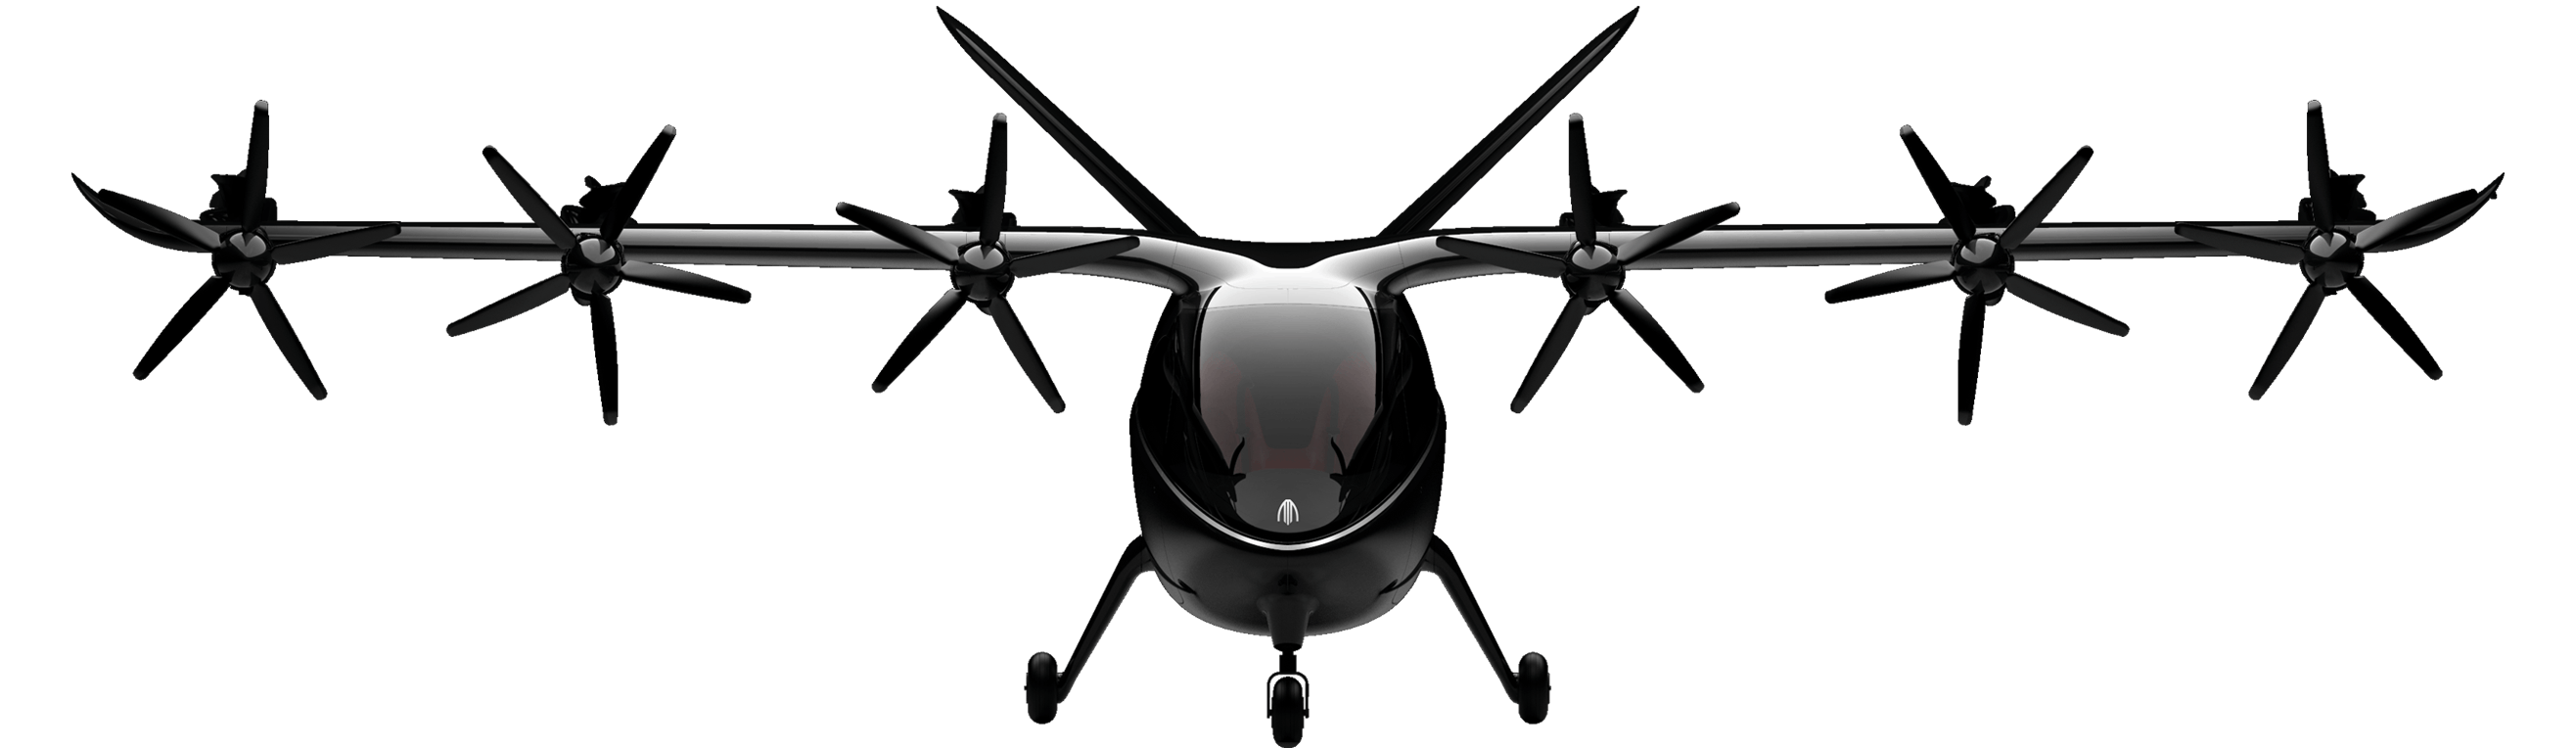
\includegraphics[scale=0.06]{Photos/archer_aircraft.png}
  }
  \quad
	\subfloat[Vahana by A$^3$ by Airbus LLC]
	{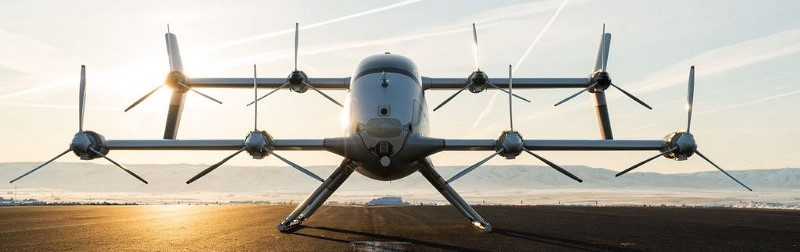
\includegraphics[scale=0.23]{Photos/Vahana.jpeg}
  }
\end{figure}

\end{frame}









%%%%%%%%%%%%%%%%%%%%%%%%%
 \section{Study Case}

   \begin{frame}
    \frametitle{Outline}
    \begin{columns}[T]
        \begin{column}{.45\textwidth}
            \tableofcontents[sections=1-3,currentsection]
        \end{column}
        \begin{column}{.45\textwidth}
            \tableofcontents[sections=4-5,currentsection]
        \end{column}
    \end{columns}
    \end{frame}

\subsection{Problem Geometry}
\begin{frame}{\subsecname}
Three-bladed propeller equipped with a left-handed Varioprop 12C 3-blades (diameter = 300 mm) \cite{tesis}  \cite{paper}.
\begin{figure} [H]  
	\centering
	\subfloat[Side-by-side]
	{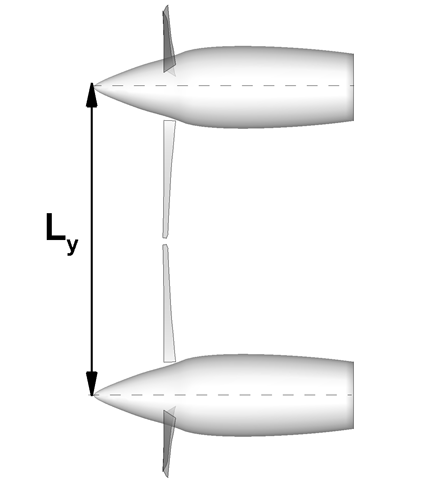
\includegraphics[scale=0.3]{Photos/side-by-side.png}
  }
  \quad
	\subfloat[Tandem]
	{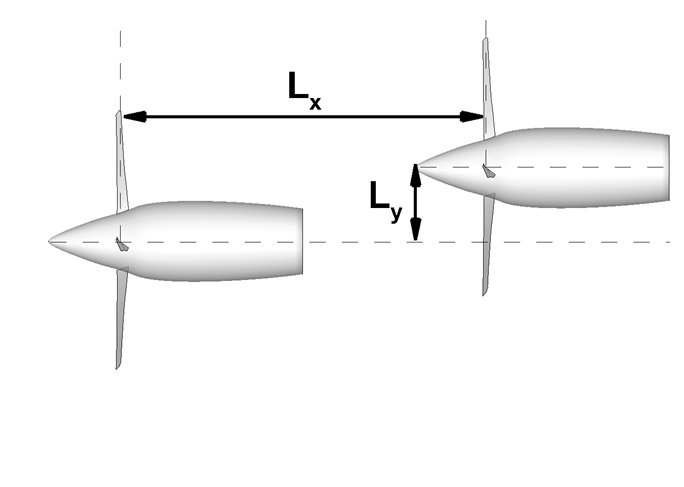
\includegraphics[scale=0.2]{Photos/tandem.png}
  }
\end{figure} 
\vspace{-0.5cm}
 \begin{table}[H]
                %\caption*{\textbf{Title of Table (optional)}}
                \centering 
                \begin{tabular}{|c c c |}
                \hline
                \rowcolor{bluePoli!40 } % bluePoli!40 comment this line to remove the color
                  & $L_x$ [m] & $L_y$ [m]  \T\B \\
                \hline \hline
                Side-by-Side Props & 0 & [0.31 0.40]\T\B  \\
                Tandem Props & 0.1 & [0.25 0.31]\T\B  \\
                \hline
                \end{tabular}
    \end{table}
\end{frame}

\begin{frame}{\subsecname}
    \begin{figure} [H]  
	\centering
	\subfloat [040.000]
	{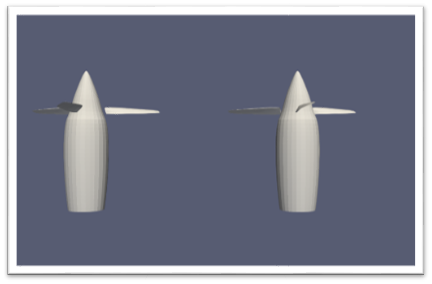
\includegraphics[scale=0.35]{Photos/040.000.png}}
  \quad
	\subfloat [031.010]
	{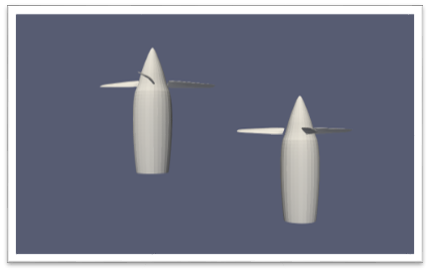
\includegraphics[scale=0.35]{Photos/031.010.png}}
  \quad
	\subfloat [031.000]
	{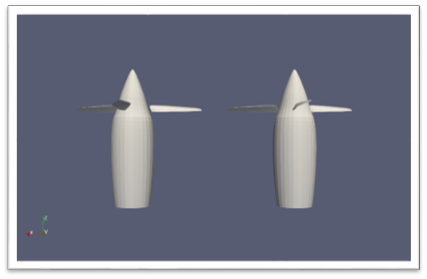
\includegraphics[scale=0.35]{Photos/031.000.png}}
   \quad
	\subfloat [025.010]
	{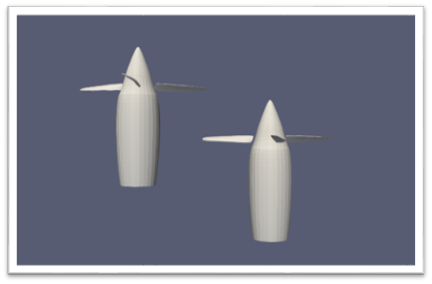
\includegraphics[scale=0.35]{Photos/025.010.png}}
\end{figure} 
\end{frame}

\subsection{Setup}
\begin{frame}{\subsecname}
\begin{itemize}
    \item $V_\inf$ = 28 m/s \& $M_a$ = 0.082
    \item $\omega$ = 738 rad/s
    \item Tip Mach Number \xrightarrow{} $M_t$ = 0.32 
    \item Propellers aligned to the freestream velocity vector
\end{itemize}
\end{frame}



\section{Methodology}
    \begin{frame}
    \frametitle{Outline}
    \begin{columns}[T]
        \begin{column}{.45\textwidth}
            \tableofcontents[sections=1-3,currentsection]
        \end{column}
        \begin{column}{.45\textwidth}
            \tableofcontents[sections=4-5,currentsection]
        \end{column}
    \end{columns}
    \end{frame}
%%%%%%%%%%%%%%%%%%%%%%%%%%%%%%%%%%%%%%%%%%%%%%%%%%%%%%%%%%%%%%%%%%%%
    \subsection{Dust}
    \begin{frame}{\subsecname}
    \begin{itemize}
        \item Novel mid-fidelity aerodynamic solver based on: 
        \begin{itemize}
            \item Vortex Particle Method (VPM) $\xrightarrow{}$ Wake modeling
            \item Lifting Line Elements $\xrightarrow{}$ Solid Boundaries
        \end{itemize} 
    \end{itemize}
    \begin{figure} [H]  
	\centering
	\subfloat
	{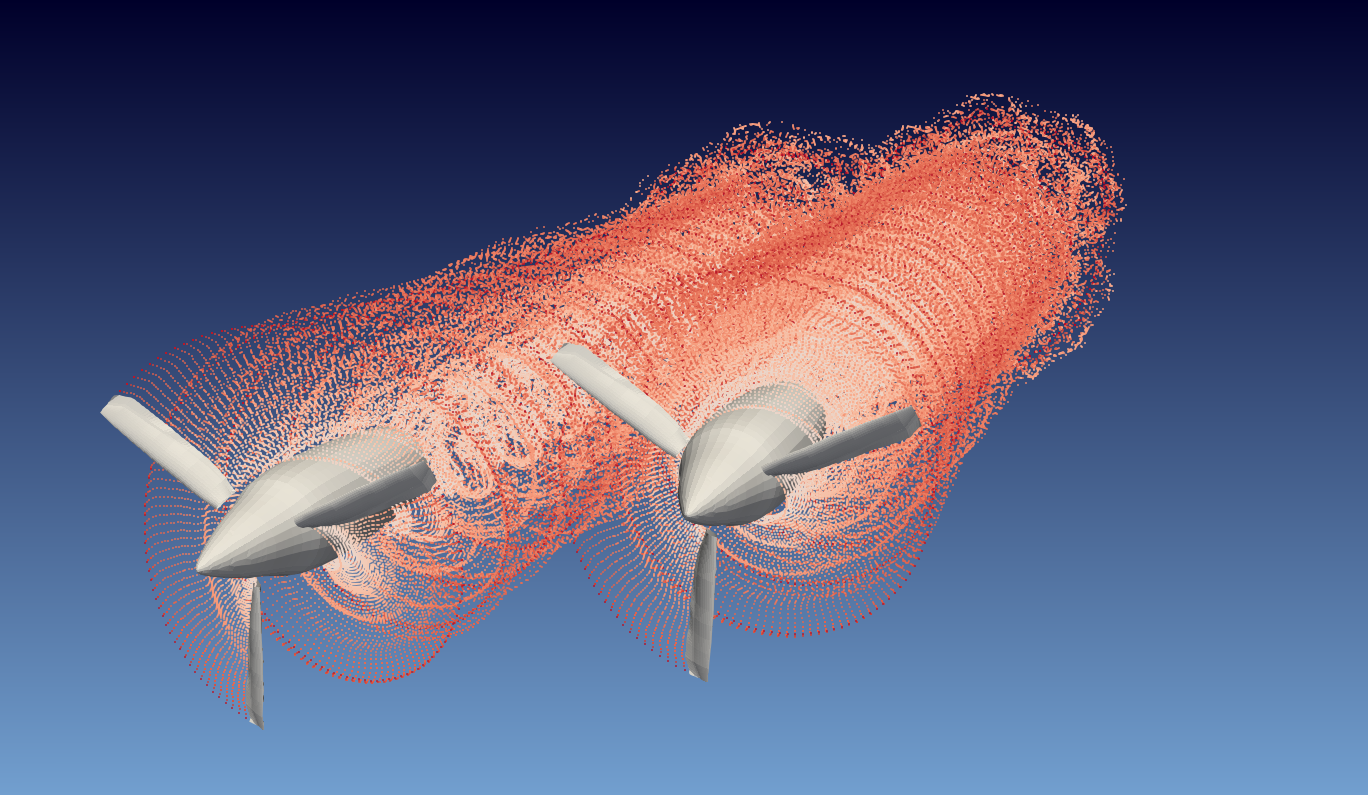
\includegraphics[scale=0.11]{Photos/2_rotors_dust_wake.eps}
  }
  \quad
	\subfloat
	{\includegraphics[scale=0.11]{Photos/2_rotors_dust__wake_side.eps}
  }
  \caption{DUST's wake visualization ($L_x$=0.1m, $L_y$=0.31m)}
\end{figure} 
    \end{frame}


\subsection{SU2 (CAA)}
\begin{frame}{\subsecname}
    \begin{itemize}
        \item FWH numeric approach
        \item Surface flow files (DUST outputs)
        \item Dummy mesh
        \item Acoustic Configuration
        \item 36 Observers, located at R = 2m:
    \end{itemize}

\begin{figure}
\subfloat [2 rotors]
	{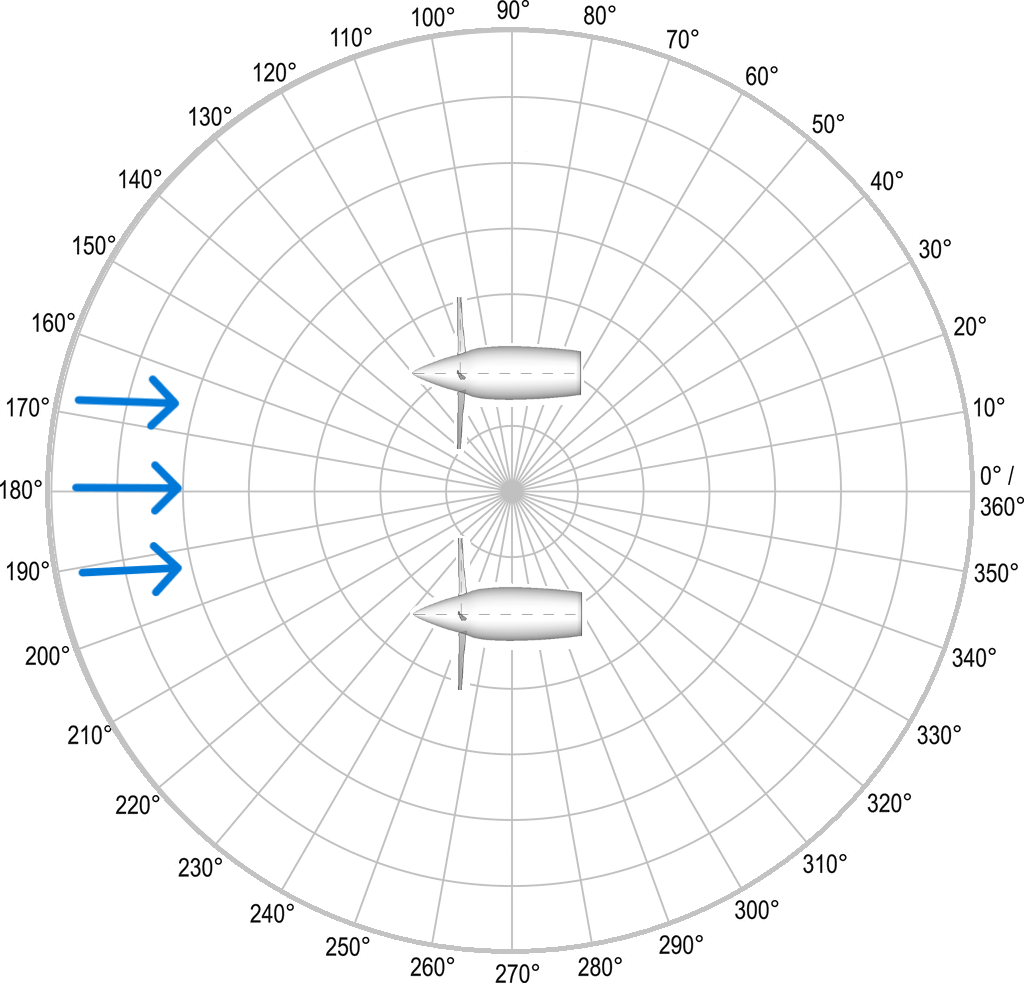
\includegraphics[scale=0.18]{Photos/observers_2rotors.png}
  }
  \quad
	\subfloat [1 rotor]
	{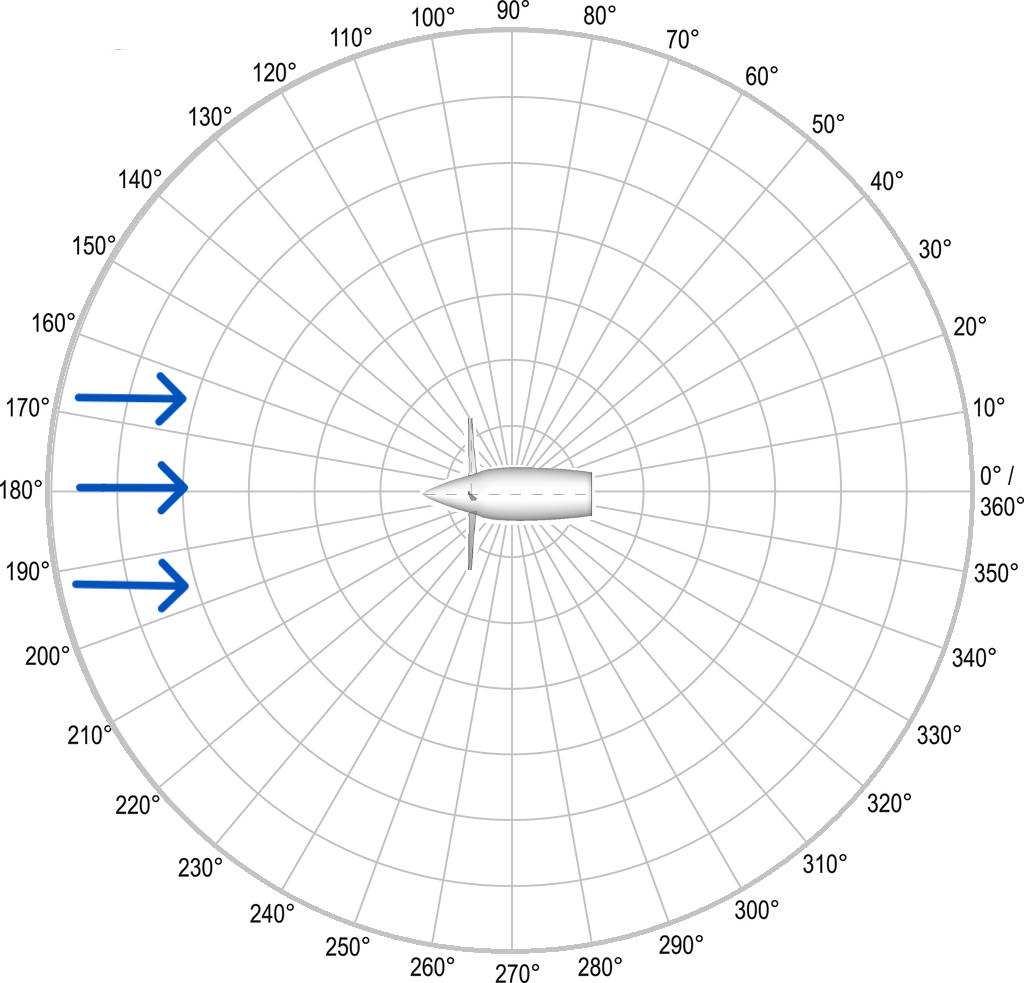
\includegraphics[scale=0.18]{Photos/observers_1rotor.png}
  }
\end{figure}

\end{frame}    



\section{Results}
    \begin{frame}
    \frametitle{Outline}
    \begin{columns}[T]
        \begin{column}{.45\textwidth}
            \tableofcontents[sections=1-3,currentsection]
        \end{column}
        \begin{column}{.45\textwidth}
            \tableofcontents[sections=4-5,currentsection]
        \end{column}
    \end{columns}
    \end{frame}

\subsection{Transitory Regime}
\begin{frame}{\subsecname}
    
\begin{figure} [H]  
	\centering
	\subfloat
	{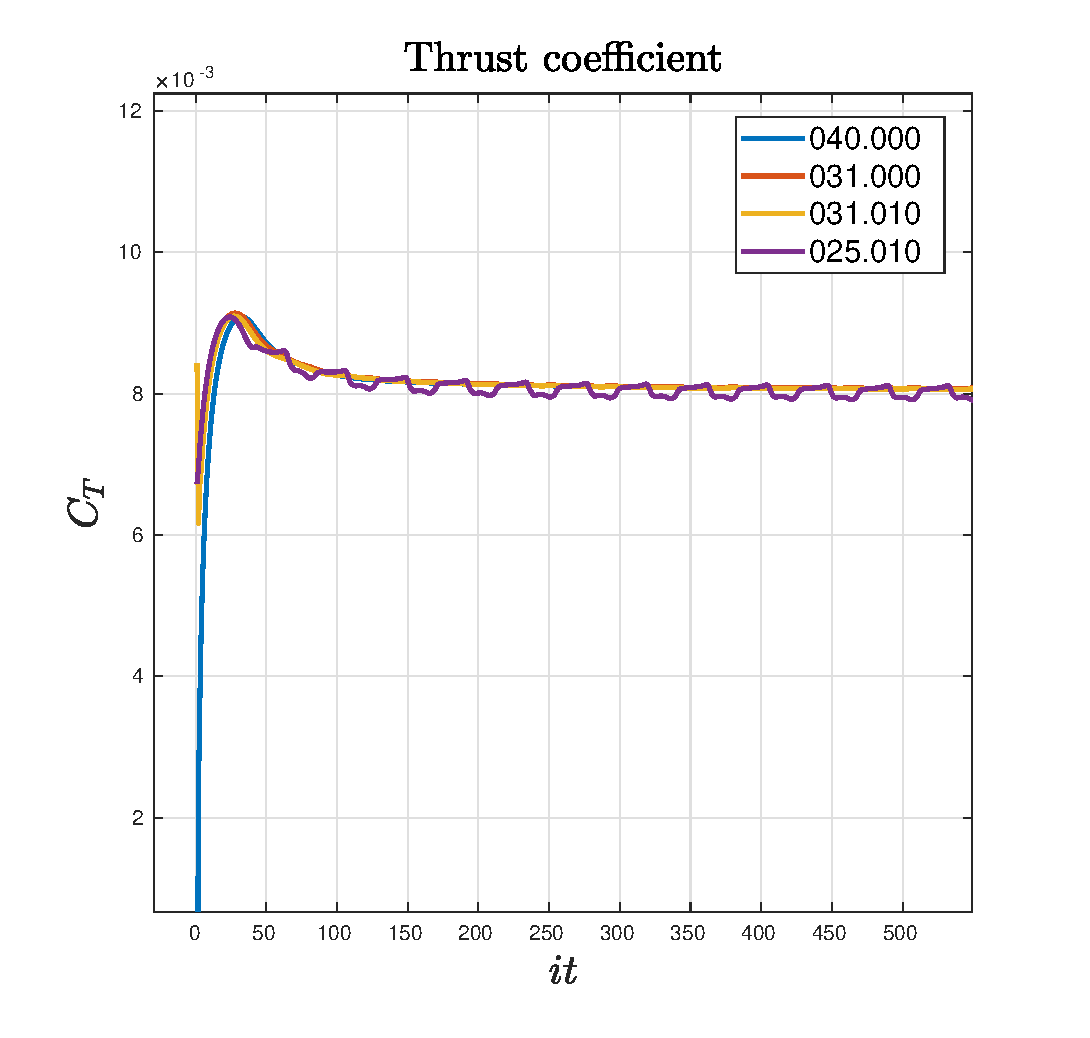
\includegraphics[scale=0.30]{Photos/Ct_iter.eps}}
  \quad
	\subfloat
	{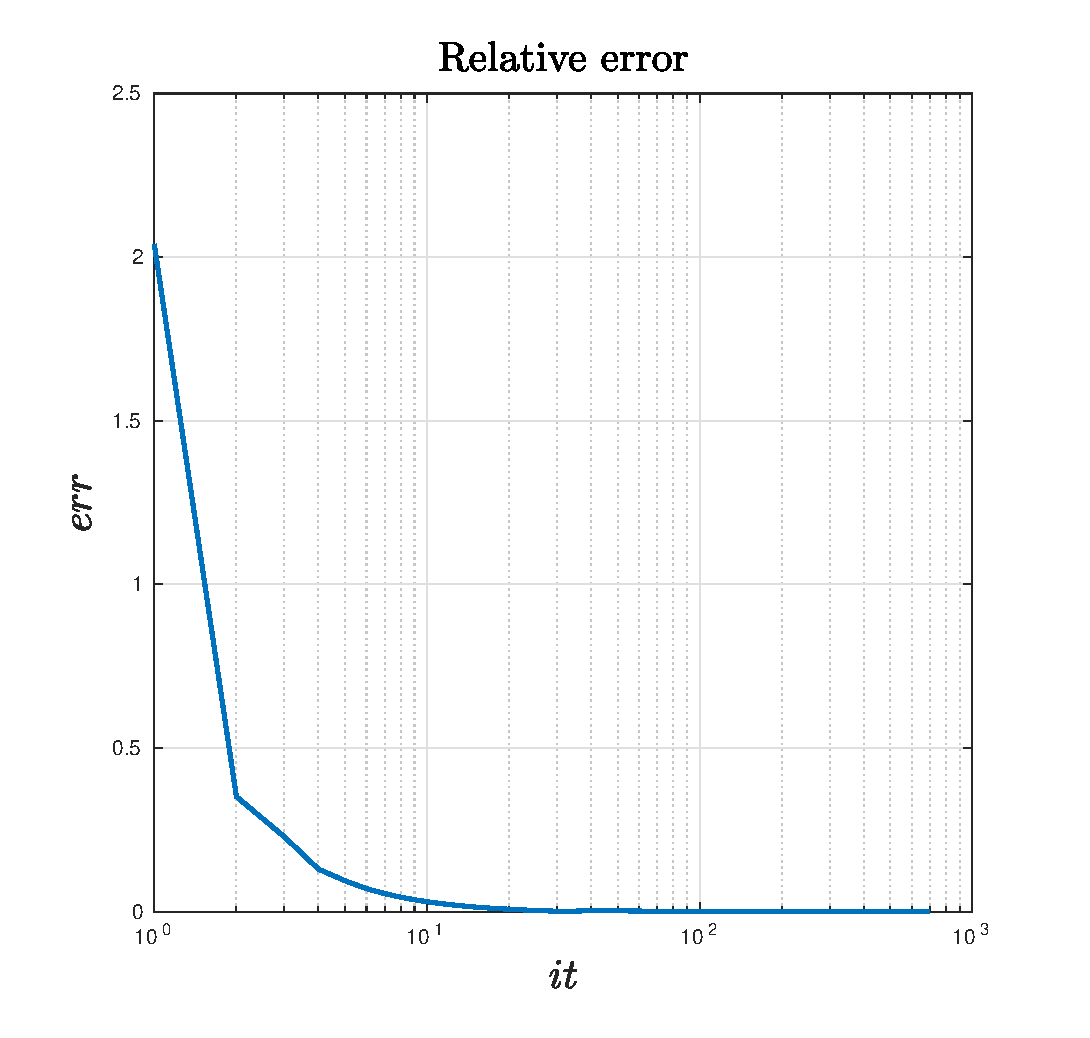
\includegraphics[scale=0.30]{Photos/err_iter.eps}
  }
\end{figure} 
\begin{center}
\vspace{-0.4cm}
 $c_T = \frac{T}{\rho n^2 D^4}$ \hspace{4cm} $err = \frac{\abs{c_T^{i+1}- c_T^{i}}}{c_T^{i+1}}$
 \newline
 \newline
    1 rev = 128 iter $\xrightarrow{}$ Stationary regime after 3 revs = 384 iter
\end{center}

\end{frame}

\subsection{SPL: Two rotors }
\begin{frame}{\subsecname}

\begin{figure} [H]  
	\centering
	\subfloat
	{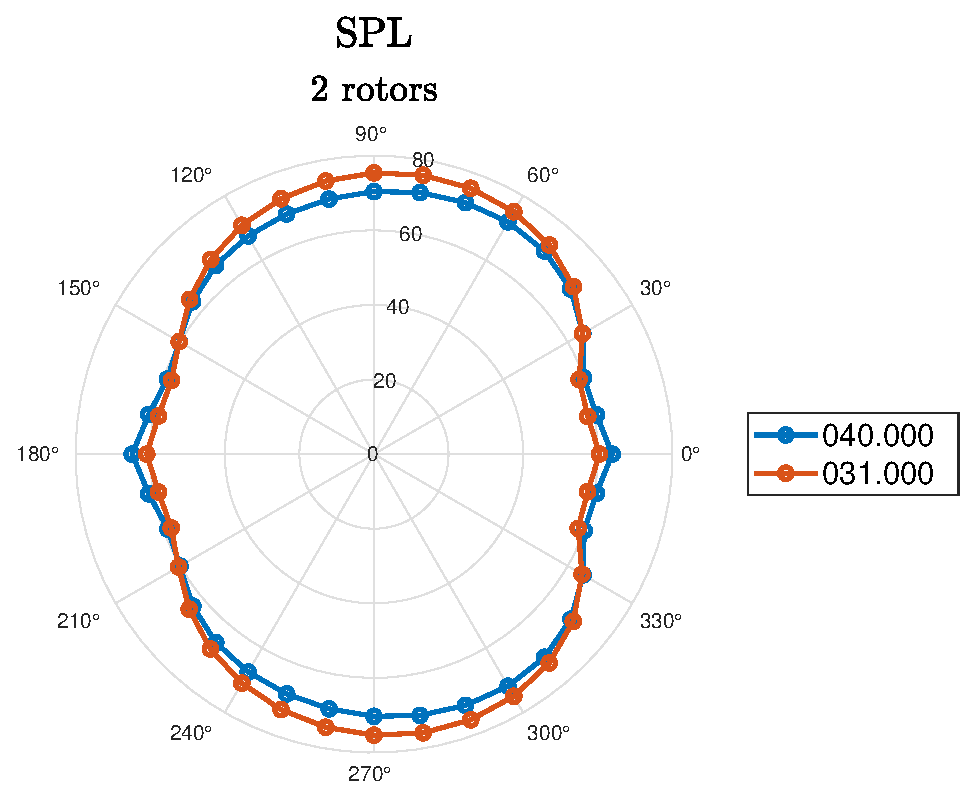
\includegraphics[scale=0.35]{Photos/spl_2rot_040000_031000.eps}}
  %\quad
	\subfloat
	{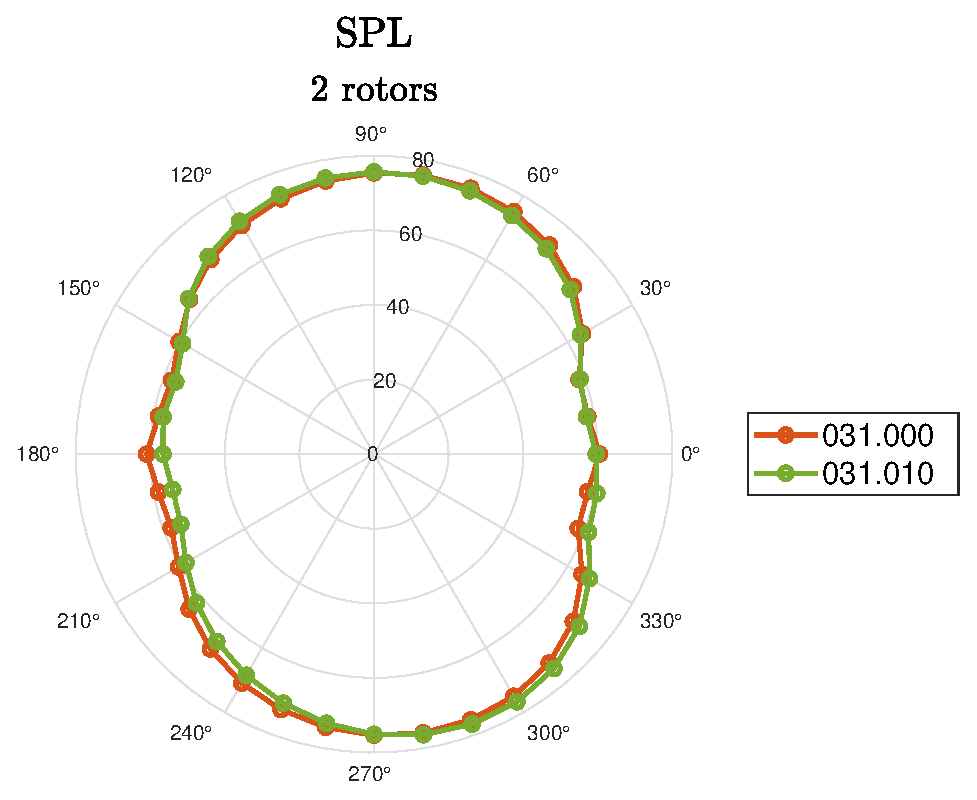
\includegraphics[scale=0.35]{Photos/spl_2rot_031000_031010.eps}
  }
\end{figure} 
\end{frame}

\begin{frame}{\subsecname}
\begin{figure} [H]  
	\centering
	\subfloat
	{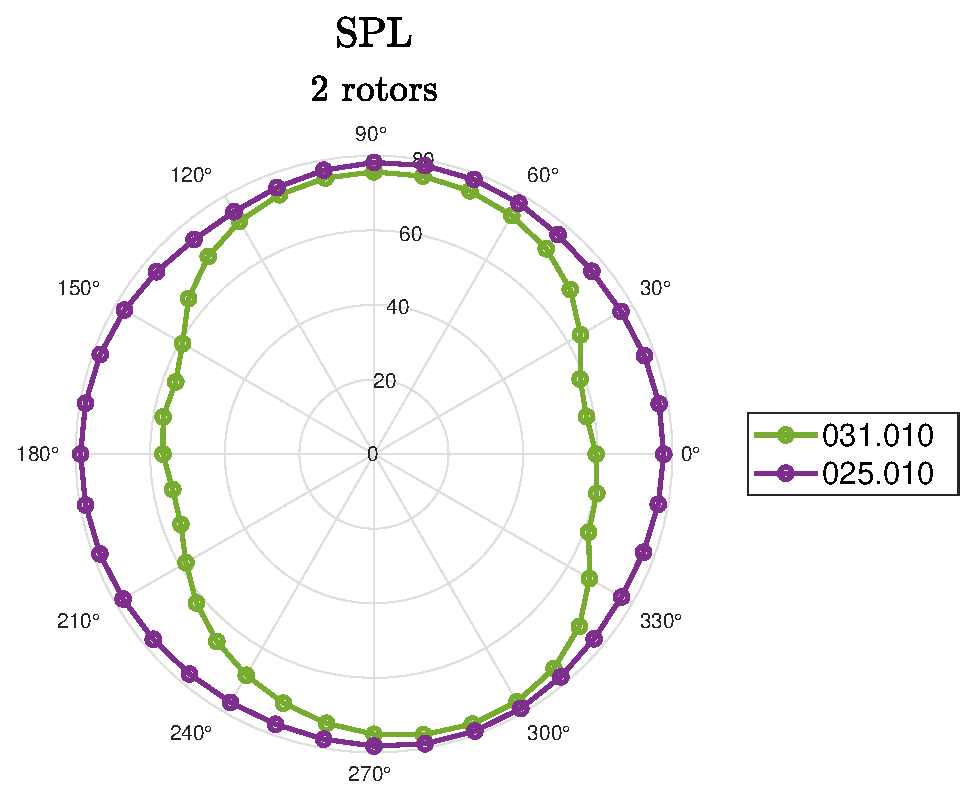
\includegraphics[scale=0.35]{Photos/spl_2rot_031010_025010.eps}}
  %\quad
	\subfloat
	{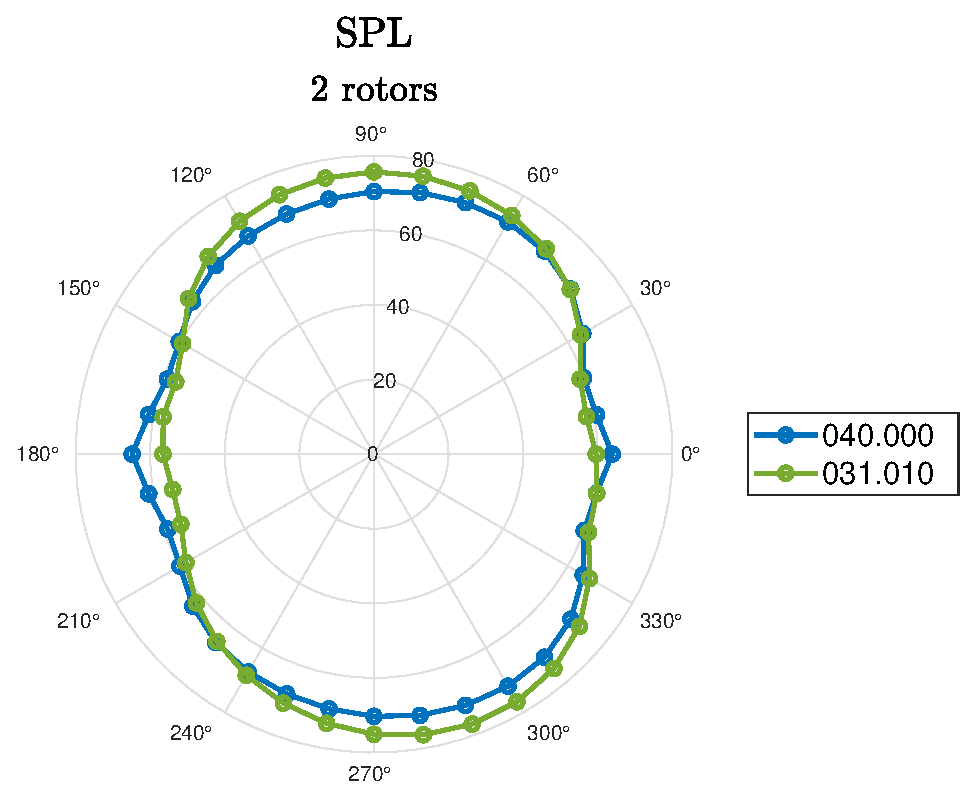
\includegraphics[scale=0.35]{Photos/spl_2rot_040000_031010.eps}
  }
\end{figure} 

\end{frame}

 \subsection{Pressure Fluctuation}
\begin{frame}{\subsecname}
    \begin{figure} [H]  
	\centering
	\subfloat [$\Delta t$ = 9.09x10$^{-4}$ s]
	{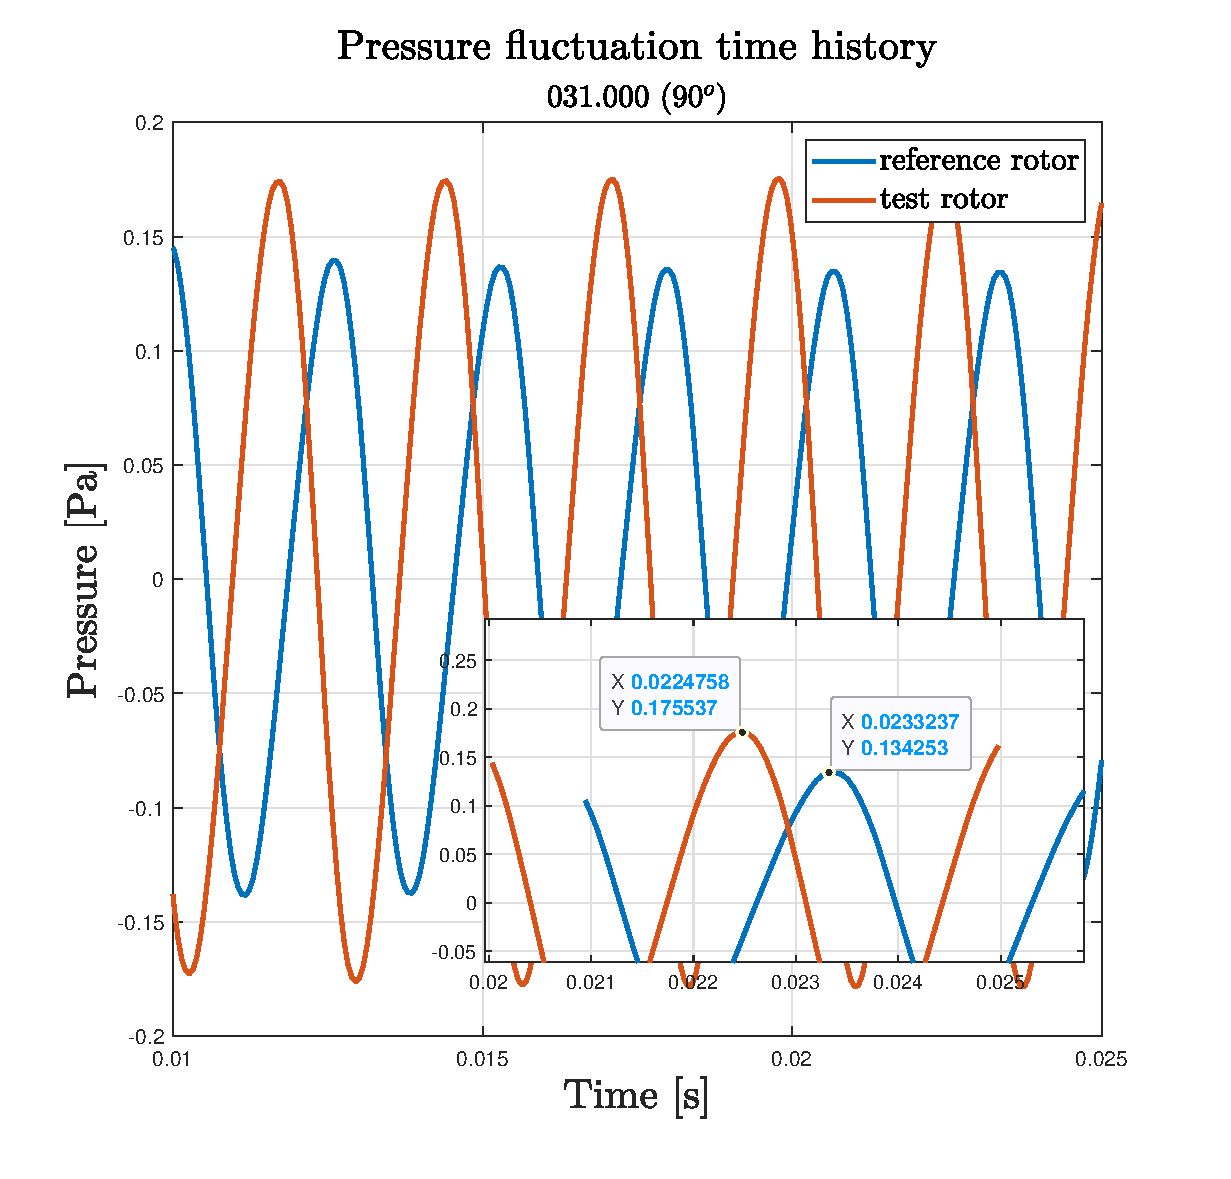
\includegraphics[scale=0.27]{Photos/phase_shift_031000.eps}}
  \quad
	\subfloat [$\Delta t$ = 1.12x10$^{-3}$ s]
	{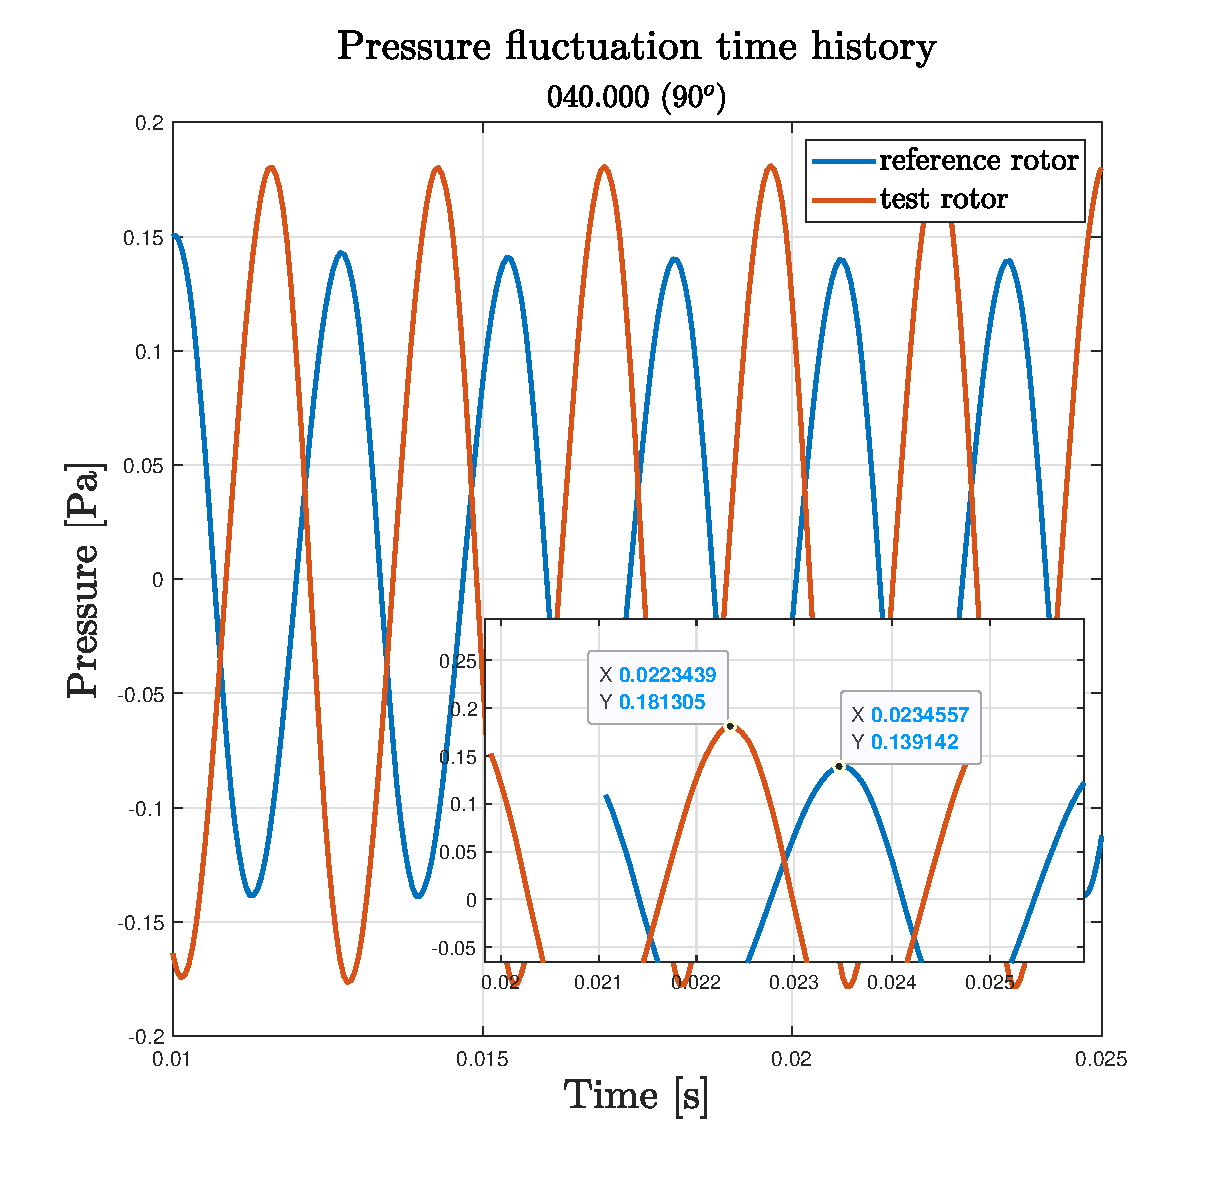
\includegraphics[scale=0.27]{Photos/phase_shift_040000.eps}
  }
\end{figure} 
    
\end{frame}

\subsection{PSD}
\begin{frame}{\subsecname}
    \begin{figure} [H]  
	\centering
	\subfloat
	{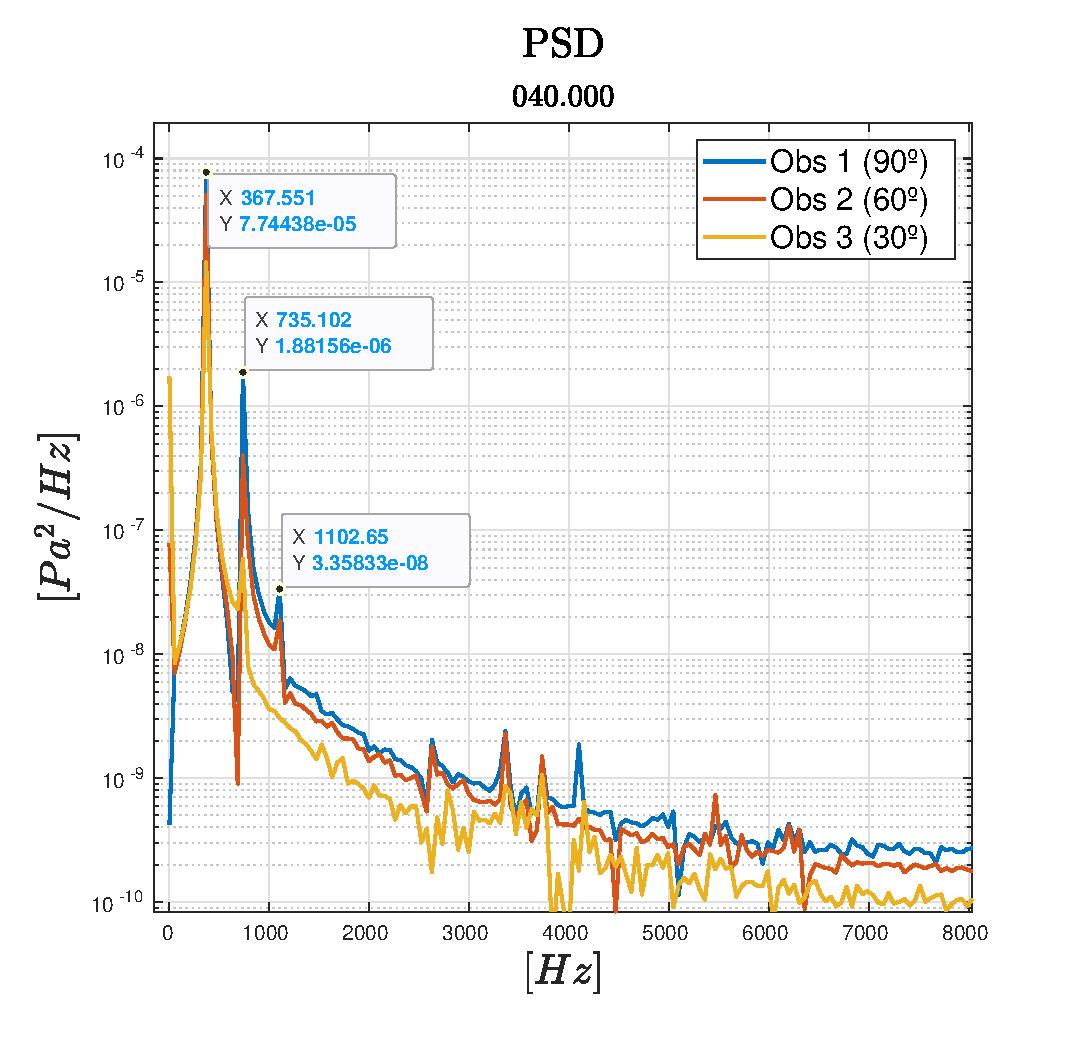
\includegraphics[scale=0.305]{Photos/psd_040000.eps}}
  \quad
	\subfloat
	{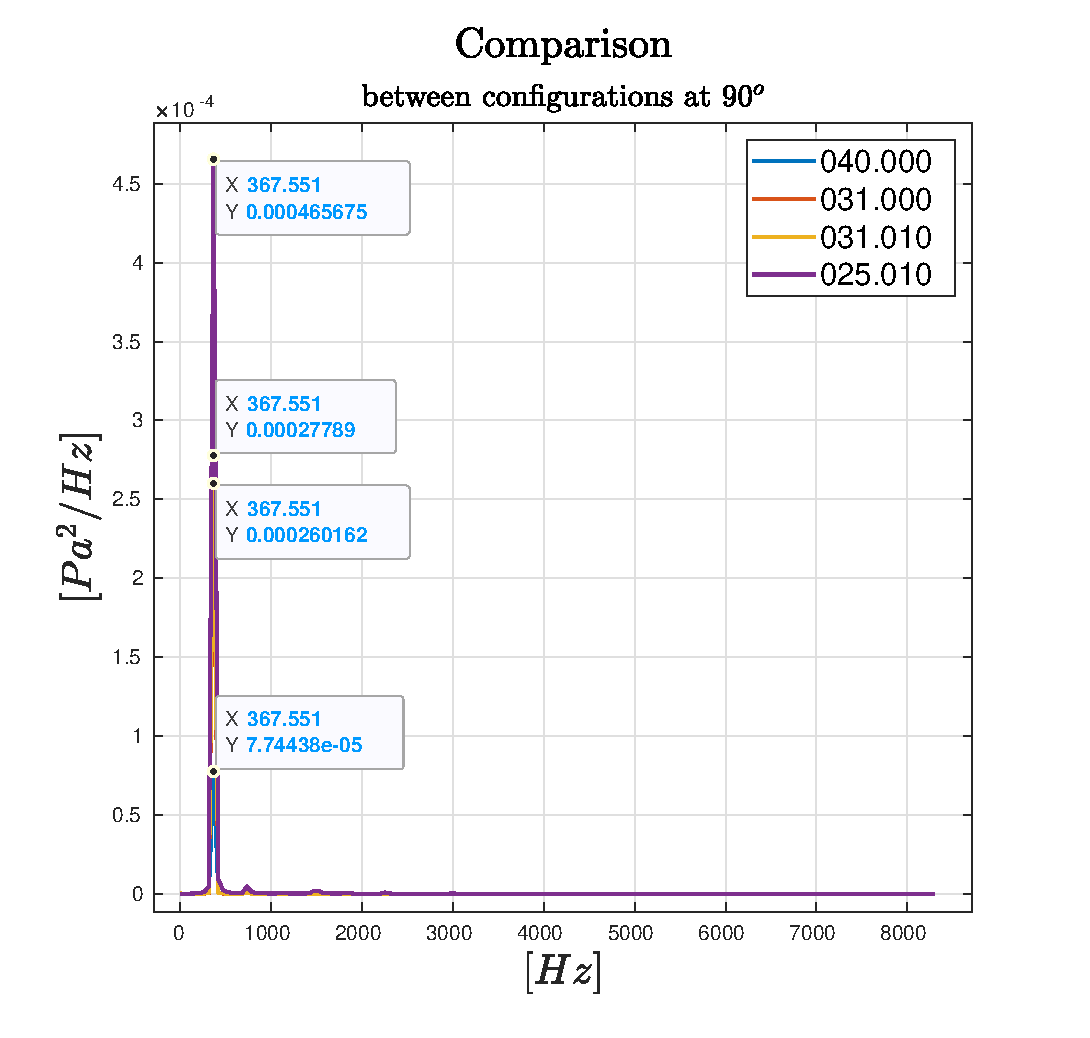
\includegraphics[scale=0.305]{Photos/psd_comparison.eps}
  }
\end{figure}
\begin{center}
    
\resizebox{8cm}{!}{
 \begin{table}[H]
                %\caption*{\textbf{Title of Table (optional)}}
                \centering 
                \begin{tabular}{|c c c |}
                \hline
                \rowcolor{bluePoli!40 } % bluePoli!40 comment this line to remove the color
                  Sampling frequency [$Hz$] & Time Step [$s$] & Signal duration [$s$]\T\B \\
                \hline \hline
                1.6726x10$^4$ & 6.6514x10$^{-5}$ & 0.08514 (10 rev)\T\B  \\
                \hline
                \end{tabular}
    \end{table}}
    \end{center}
\end{frame}



\subsection{SPL: One rotor}
\begin{frame}{\subsecname}
    \begin{figure} [H]  
	\centering
	\subfloat
	{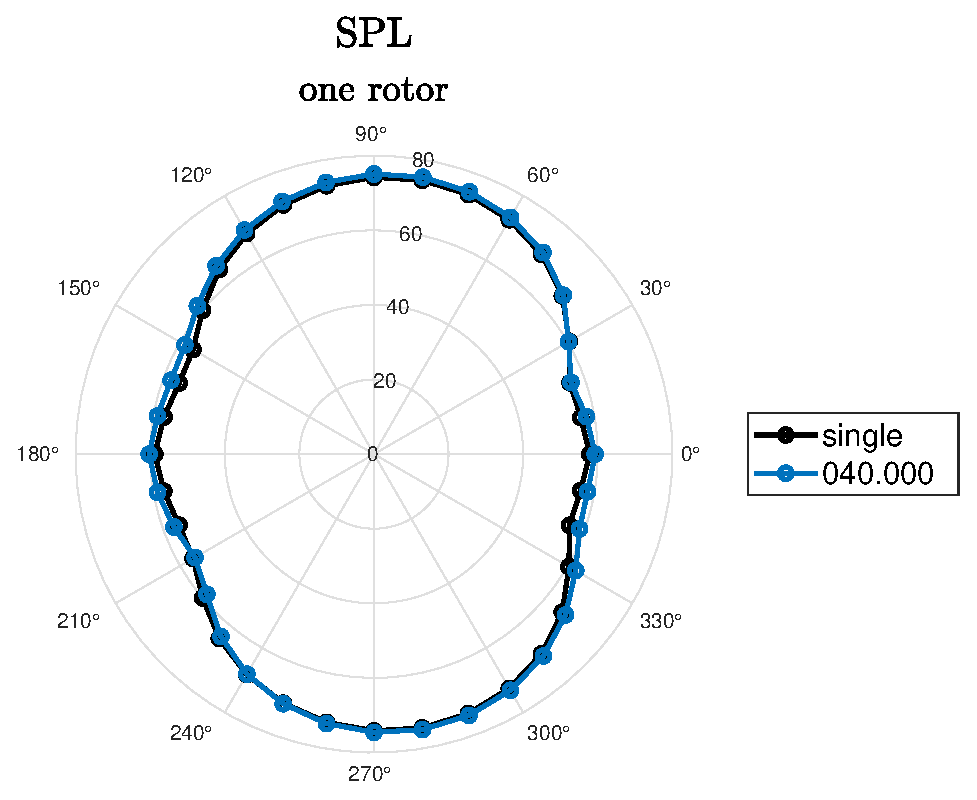
\includegraphics[scale=0.35]{Photos/spl_1rot_040000_single.eps}}
 % \quad
	\subfloat
	{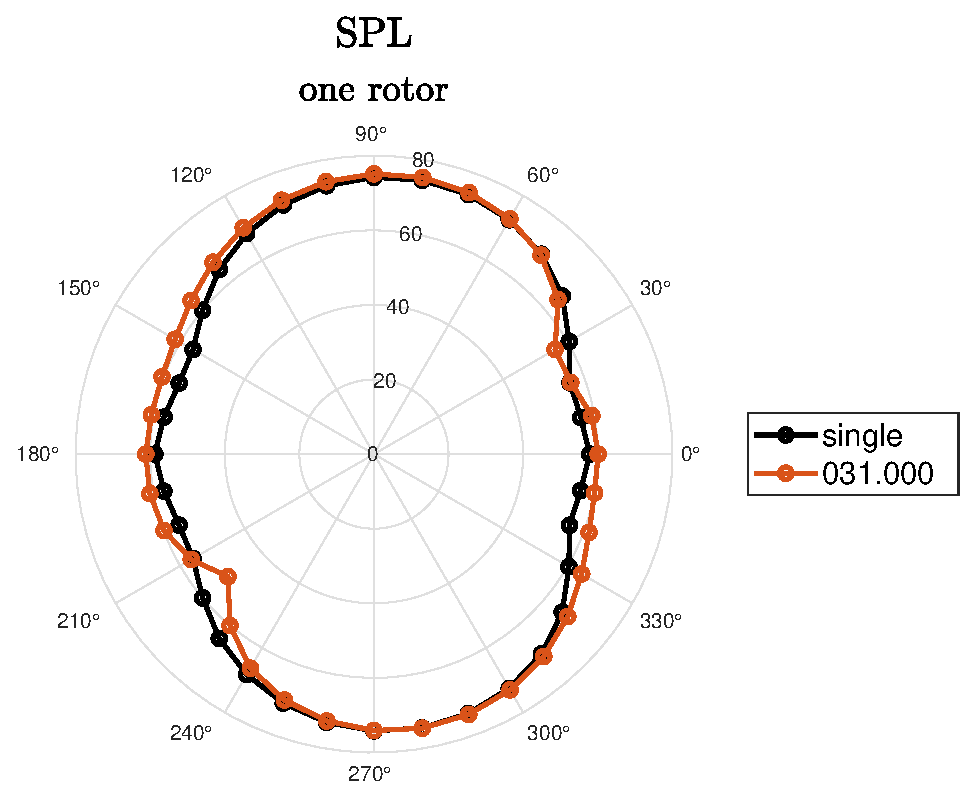
\includegraphics[scale=0.35]{Photos/spl_1rot_031000_single.eps}
  }
\end{figure} 
\end{frame}

\begin{frame}{\subsecname}
    \begin{figure} [H]  
	\centering
	\subfloat
	{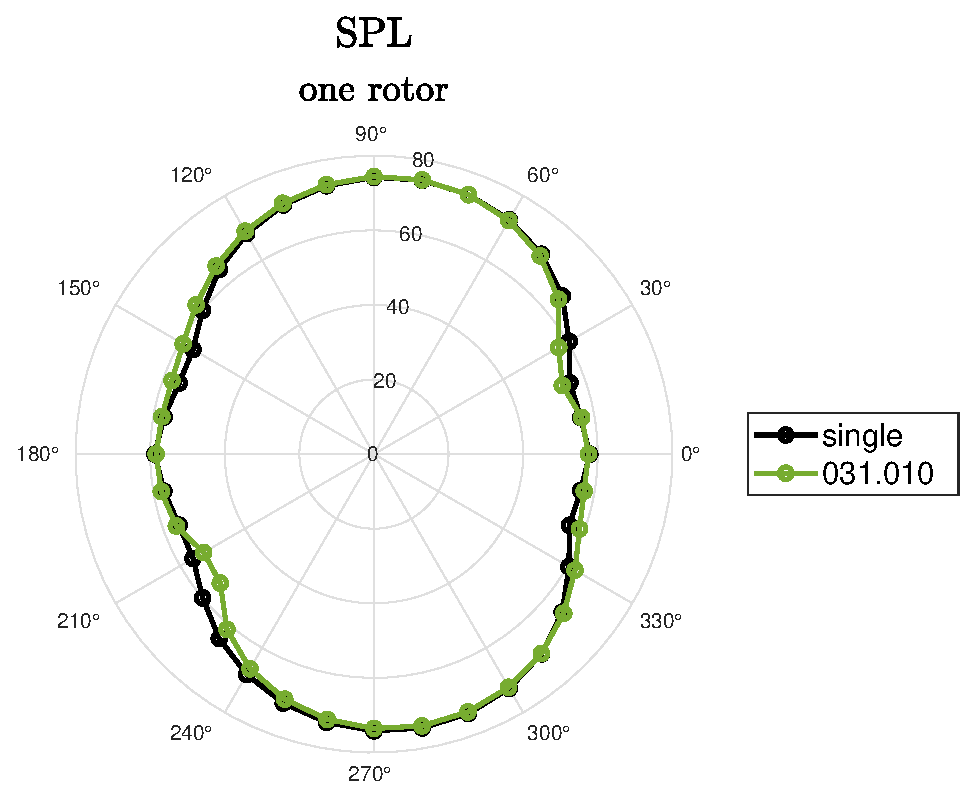
\includegraphics[scale=0.35]{Photos/spl_1rot_031010_single.eps}}
 % \quad
	\subfloat
	{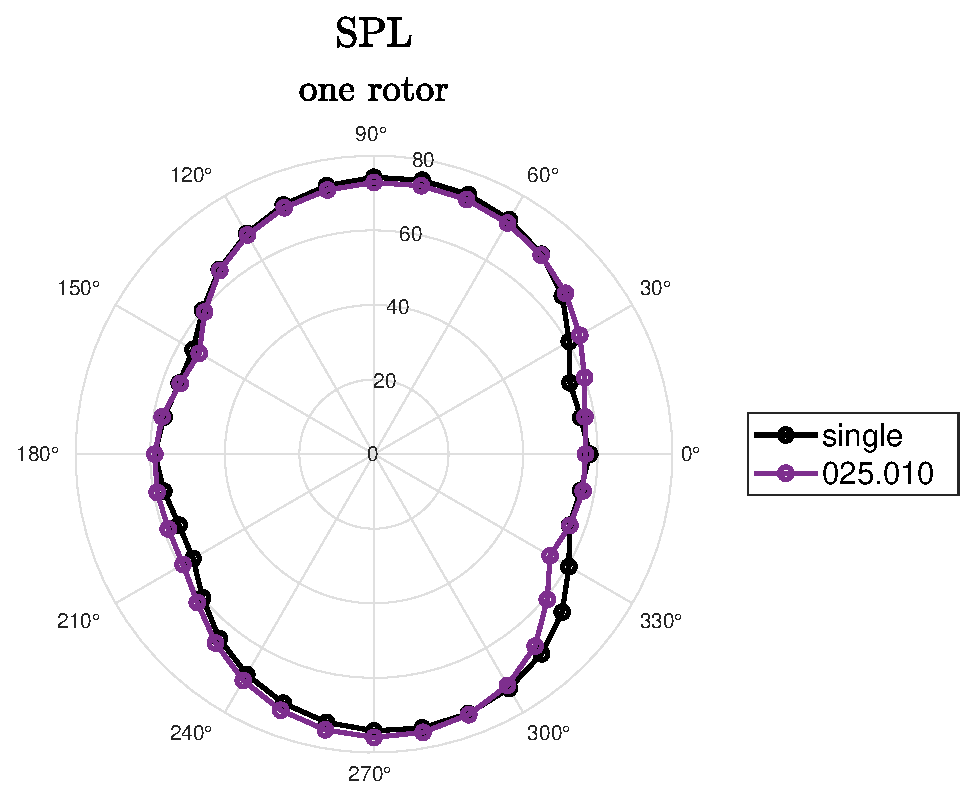
\includegraphics[scale=0.35]{Photos/spl_1rot_025010_single.eps}}
\end{figure} 
\end{frame}

\subsection{Tonal Noise: One rotor}
\begin{frame}{\subsecname}
    \begin{figure} [H]  
	\centering
	\subfloat
	{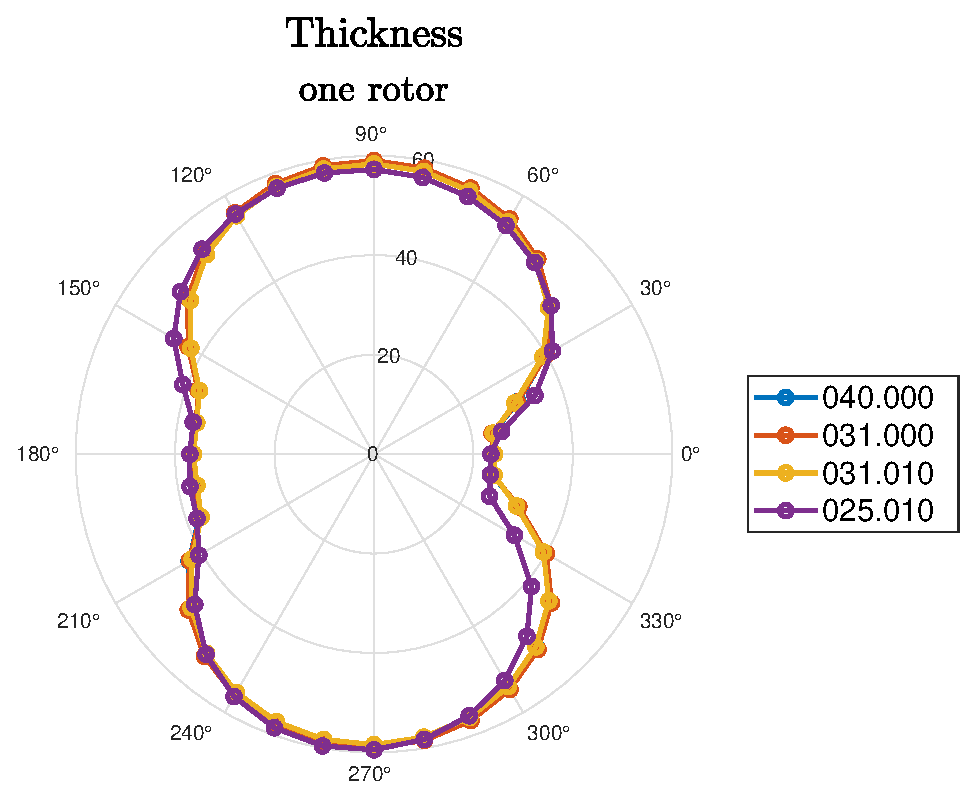
\includegraphics[scale=0.35]{Photos/thickness_comparison.eps}}
  %\quad
	\subfloat
	{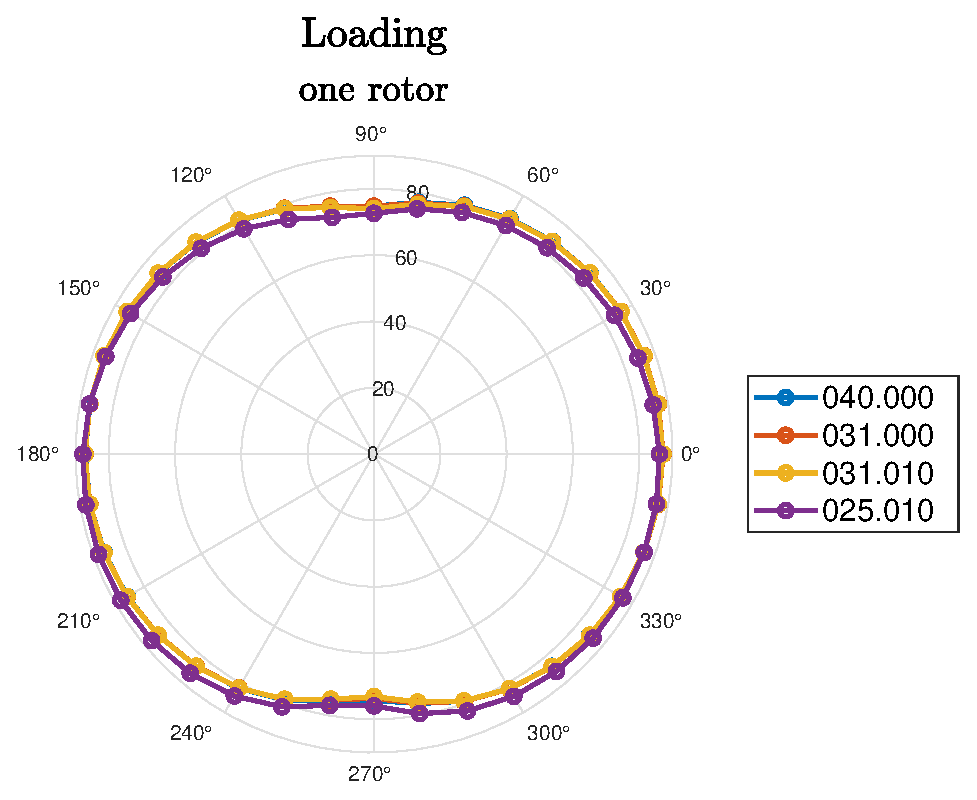
\includegraphics[scale=0.35]{Photos/loading_comparison.eps}
  }
\end{figure} 
\end{frame}


\section{Conclusions}
    \begin{frame}
    \frametitle{Outline}
    \begin{columns}[T]
        \begin{column}{.45\textwidth}
            \tableofcontents[sections=1-3,currentsection]
        \end{column}
        \begin{column}{.45\textwidth}
            \tableofcontents[sections=4-5,currentsection]
        \end{column}
    \end{columns}
    \end{frame}


\subsection{Configurations Comparison}
\begin{frame}{\subsecname}

\begin{minipage}[t]{0.5\linewidth}
\begin{figure}[H]
    \centering
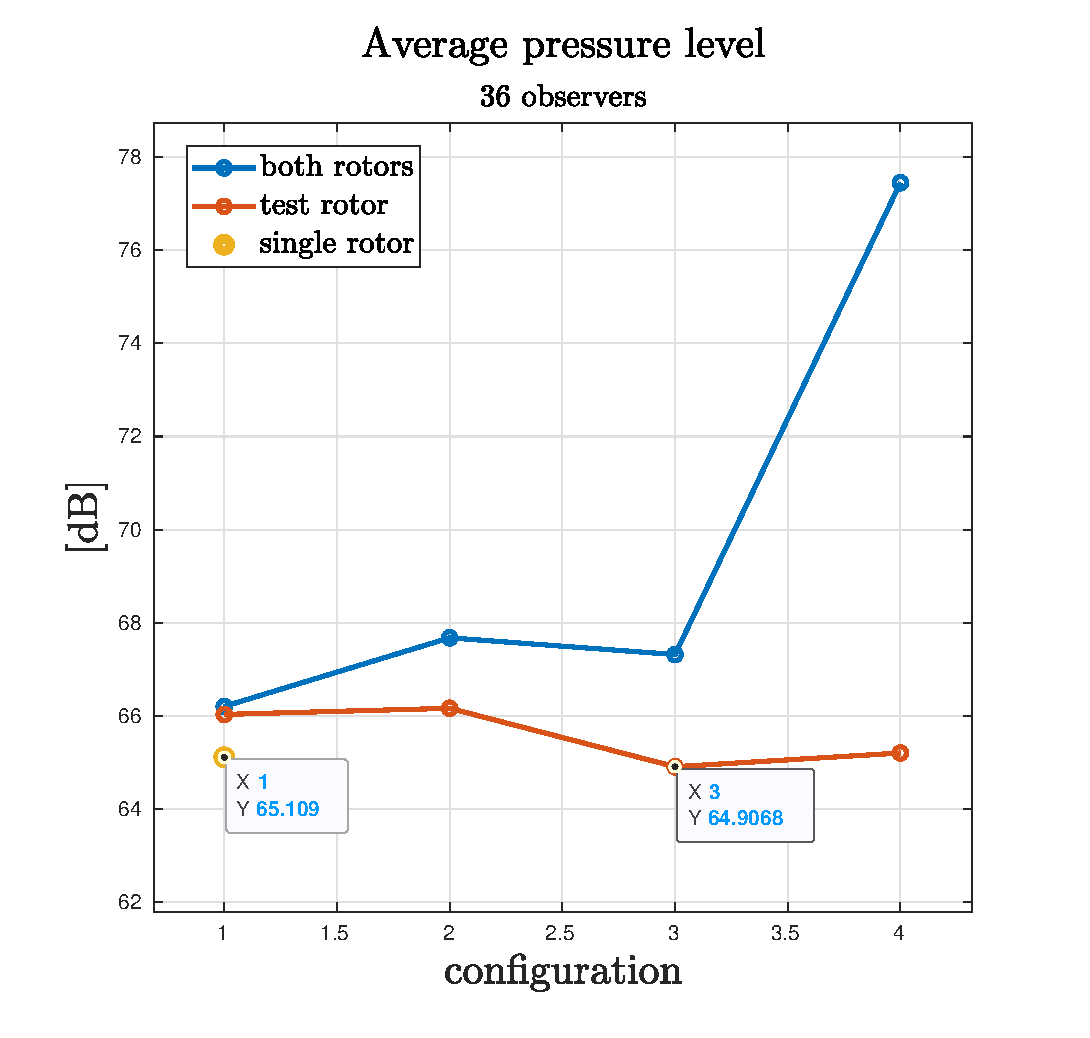
\includegraphics[scale=0.36]{Photos/averageSPL_config_comparison.eps}
\end{figure}  
\end{minipage}\hfill
\begin{minipage}[t]{0.43\linewidth}
\vspace{2cm}
\resizebox{5cm}{!}{
 \begin{table}[H]
                %\caption*{\textbf{Title of Table (optional)}}
                \centering 
                \begin{tabular}{|c c c|}
                \hline
                \rowcolor{bluePoli!40 } % bluePoli!40 comment this line to remove the color
                Config & 1 rotor [dB] & 2 rotors [dB] \T\B \\
                \hline \hline
                1 (040.000) & 66.03  & 66.20 \T\B  \\
                2 (031.000) & 66.16 & 67.68 \T\B  \\
                3 (030.010) & 64.91 & 67.32 \T\B  \\
                4 (025.010) & 65.20 & 77.45 \T\B  \\
                \hline \hline
                Single Rotor & 65.11 & \T\B  \\
                \hline
                \end{tabular}
    \end{table} }
    
\end{minipage}





\end{frame}


\begin{frame}
   \begin{itemize}
       \item Sound gets \textbf{reduced} with:
       \begin{itemize}
        \item Increasing rotor axis distance
        \item Adding a stagger
       \end{itemize}

       \item Sound gets \textbf{amplified} when Blade Vortex Interaction occurs

       \item \textbf{Aerodynamic performance}:
       \begin{itemize}
           \item Similar behavior for non-wake interference configurations
           \item The more the wake interaction, the more reduction in performance
       \end{itemize}

       \item \textbf{Tonal Noise} is attributed to the Blade Passing Frequency

       
   \end{itemize}
\end{frame}

 \subsection{Further Investigation}
 \begin{frame} {\subsecname}
     \begin{itemize}
         \item Observers located in the vertical plane
         \item Changing the stagger distance $\xrightarrow{}$ Find the optimal configuration
         \item Validation with numerical or experimental data
         \item Aeroacoustic study of the nacelles' influence
     \end{itemize}
 \end{frame}

\subsection{Preliminary nacelle results}

\begin{frame} {\subsecname}
    \begin{figure}
\centering
\begin{minipage}{.5\textwidth}
  \centering
  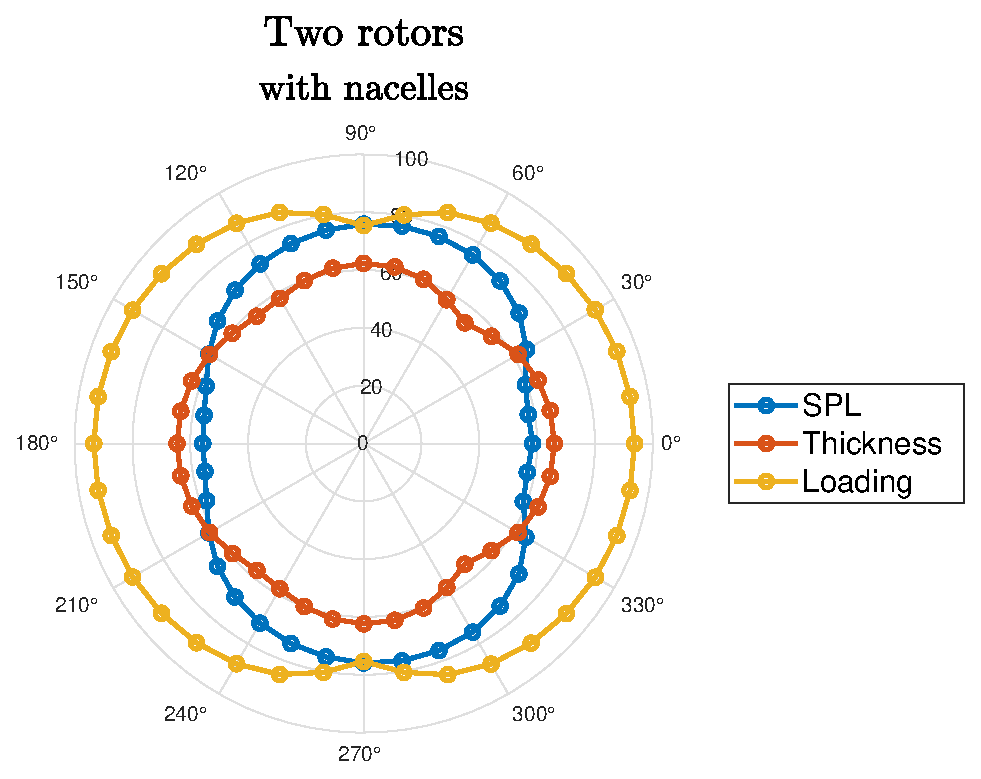
\includegraphics[scale=0.35]{Photos/spl_thick_load_nacelles.eps}
\end{minipage}%
\begin{minipage}{.5\textwidth}
  \centering
  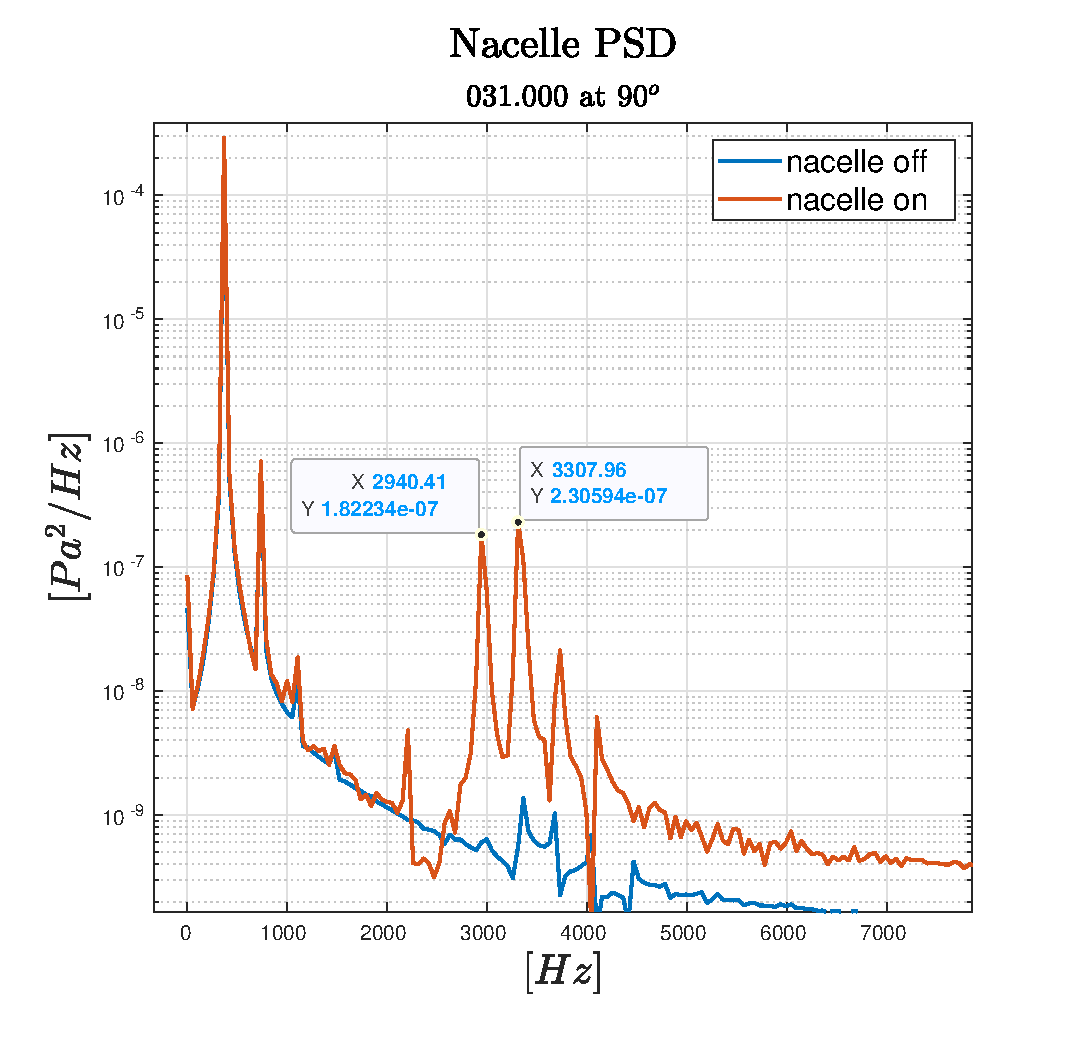
\includegraphics[scale=0.35]{Photos/psd_nacelle.eps}
\end{minipage}
\end{figure}
\end{frame}

\section{Reference Papers}
\begin{frame}
    \cite{tesis}  Algarotti, D. \textbf{Experimental-Numerical Investigation of the Aerodynamic Interaction between Tandem Propellers in eVTOL Airplane Mode}. Scuola di Ingegneria Industriale e dell'Informazione \newline
    \newline
     \cite{paper} Piccinini, R.; Tugnoli, M.; Zanotti, A. \textbf{Numerical Investigation of the Rotor-Rotor Aerodynamic Interaction for eVTOL Aircraft Configurations}. Energies 2020, 13, 5995.

\end{frame}

\begin{frame}
    \begin{figure}[H]
    \centering
\includegraphics[scale=0.07]{Photos/IMG_20230604_142810.jpg}
\end{figure}  
\end{frame}

\end{document}
